% Forward propagation practice problem (sign hidden layer, softmax output): problem and solution.
% Written in the class convention: column vectors, z = W x + b, row j of W holds the weights into node j.
% Build: pdflatex fwdprop_practice_solution.tex
\documentclass[11pt]{article}
\usepackage[margin=1in]{geometry}
\usepackage{amsmath,amssymb,bm,tikz}
\usepackage{array}
\setlength{\parindent}{0pt}
\setlength{\parskip}{6pt}
\pagestyle{empty}

\begin{document}

{\Large\bfseries Forward propagation practice problem: solution}

\begin{center}
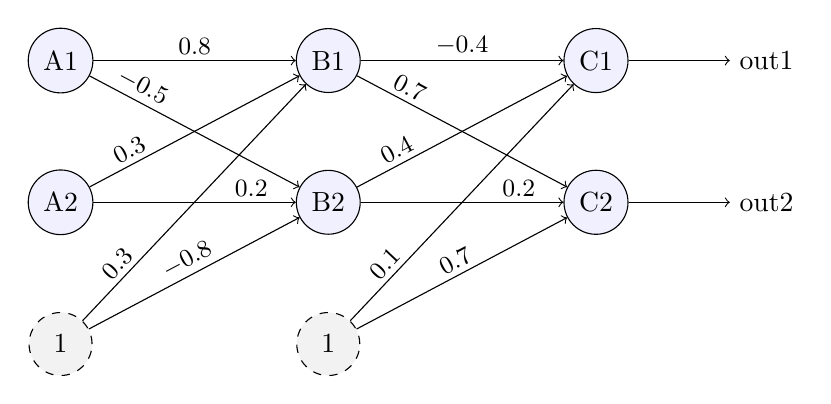
\begin{tikzpicture}[x=3.4cm,y=1.8cm,n/.style={circle,draw,minimum size=8mm,fill=blue!6},
  bn/.style={circle,draw,dashed,minimum size=8mm,fill=gray!10},
  w/.style={font=\small,fill=white,inner sep=1pt,sloped,above=1pt}]
\node[n] (A1) at (0,2) {A1}; \node[n] (A2) at (0,1) {A2}; \node[bn] (A0) at (0,0) {1};
\node[n] (B1) at (1,2) {B1}; \node[n] (B2) at (1,1) {B2}; \node[bn] (B0) at (1,0) {1};
\node[n] (C1) at (2,2) {C1}; \node[n] (C2) at (2,1) {C2};
\draw[->] (A1) -- node[w,pos=0.5] {0.8} (B1);
\draw[->] (A1) -- node[w,pos=0.22] {$-0.5$} (B2);
\draw[->] (A2) -- node[w,pos=0.22] {0.3} (B1);
\draw[->] (A2) -- node[w,pos=0.78] {0.2} (B2);
\draw[->] (A0) -- node[w,pos=0.2] {0.3} (B1);
\draw[->] (A0) -- node[w,pos=0.5] {$-0.8$} (B2);
\draw[->] (B1) -- node[w,pos=0.5] {$-0.4$} (C1);
\draw[->] (B1) -- node[w,pos=0.22] {0.7} (C2);
\draw[->] (B2) -- node[w,pos=0.22] {0.4} (C1);
\draw[->] (B2) -- node[w,pos=0.78] {0.2} (C2);
\draw[->] (B0) -- node[w,pos=0.2] {0.1} (C1);
\draw[->] (B0) -- node[w,pos=0.5] {0.7} (C2);
\draw[->] (C1) -- ++(0.5,0) node[right] {out1}; \draw[->] (C2) -- ++(0.5,0) node[right] {out2};
\end{tikzpicture}
\end{center}

\textbf{Problem.} For the network above, out1 represents Class A and out2 represents Class B.
Layer B uses the sign function as its activation, and layer C uses the softmax function. Show the
forward pass, in matrix form, of the record with Feature1 $= 5$ and Feature2 $= 10$. How would this
network classify the record (Class A or Class B)?

\textbf{Notation.} Row $j$ of a weight matrix $\bm{W}^{(l)}$ holds the weights into node $j$ of layer
$l$: $W^{(l)}_{ji}$ is the weight from node $i$ of the previous layer to node $j$. The bias of node $j$
is $b^{(l)}_j$, the weight on the input that is always 1. Vectors are columns.

\subsection*{Solution}

\textbf{Weights, read from the diagram.}
\[
\bm{W}^{(1)} = \begin{pmatrix} 0.8 & 0.3 \\ -0.5 & 0.2 \end{pmatrix}, \quad
\bm{b}^{(1)} = \begin{pmatrix} 0.3 \\ -0.8 \end{pmatrix}, \qquad
\bm{W}^{(2)} = \begin{pmatrix} -0.4 & 0.4 \\ 0.7 & 0.2 \end{pmatrix}, \quad
\bm{b}^{(2)} = \begin{pmatrix} 0.1 \\ 0.7 \end{pmatrix}.
\]
For example, the first row of $\bm{W}^{(1)}$ holds the weights into B1: 0.8 from A1 and 0.3 from A2.

\textbf{A to B.} The input is $\bm{x} = (5, 10)^\top$.
\[
\bm{z}_B = \bm{W}^{(1)} \bm{x} + \bm{b}^{(1)}
= \begin{pmatrix} 0.8 & 0.3 \\ -0.5 & 0.2 \end{pmatrix} \begin{pmatrix} 5 \\ 10 \end{pmatrix}
+ \begin{pmatrix} 0.3 \\ -0.8 \end{pmatrix}
= \begin{pmatrix} 0.8 \cdot 5 + 0.3 \cdot 10 + 0.3 \\ -0.5 \cdot 5 + 0.2 \cdot 10 - 0.8 \end{pmatrix}
= \begin{pmatrix} 7.3 \\ -1.3 \end{pmatrix}.
\]
The sign function gives $+1$ for a positive input and $-1$ for a negative one:
\[
\bm{B} = \operatorname{sign}(\bm{z}_B) = \begin{pmatrix} 1 \\ -1 \end{pmatrix}.
\]

\textbf{B to C.}
\[
\bm{z}_C = \bm{W}^{(2)} \bm{B} + \bm{b}^{(2)}
= \begin{pmatrix} -0.4 & 0.4 \\ 0.7 & 0.2 \end{pmatrix} \begin{pmatrix} 1 \\ -1 \end{pmatrix}
+ \begin{pmatrix} 0.1 \\ 0.7 \end{pmatrix}
= \begin{pmatrix} -0.4 \cdot 1 + 0.4 \cdot (-1) + 0.1 \\ 0.7 \cdot 1 + 0.2 \cdot (-1) + 0.7 \end{pmatrix}
= \begin{pmatrix} -0.7 \\ 1.2 \end{pmatrix}.
\]
The softmax turns these scores into probabilities. With $e^{-0.7} = 0.4966$ and $e^{1.2} = 3.3201$,
\[
\bm{C} = \operatorname{softmax}(\bm{z}_C)
= \frac{1}{e^{-0.7} + e^{1.2}} \begin{pmatrix} e^{-0.7} \\ e^{1.2} \end{pmatrix}
= \frac{1}{3.8167} \begin{pmatrix} 0.4966 \\ 3.3201 \end{pmatrix}
= \begin{pmatrix} 0.1301 \\ 0.8699 \end{pmatrix}.
\]

\textbf{Classification.} out1 $= 0.1301$ (Class A) and out2 $= 0.8699$ (Class B). The larger output is
out2, so the network classifies the record as \textbf{Class B}.

\end{document}
